\documentclass{beamer}
\usetheme{CambridgeUS}
\usecolortheme{beaver}

\newcommand\hmmax{0}
\newcommand\bmmax{0}

\usepackage{stmaryrd}

\usepackage{amsmath,amssymb,enumerate,amsthm}
\usepackage{bm}
\usepackage{graphicx}

\usepackage{algorithm, algpseudocode}
\usepackage[strict]{siunitx}
\usepackage{hyperref}
\usepackage{mathrsfs}

\usepackage{bm}
\usepackage{empheq}
\usepackage{cleveref}
\usepackage{xcolor}
\usepackage{textcomp}
\usepackage{siunitx}
\usepackage{booktabs}
\usepackage{caption}
\usepackage{tikz}
\usetikzlibrary{decorations.pathreplacing,calligraphy}
\usepackage{pgfplots}
\NewDocumentCommand{\R}{}{\mathbb{R}}
\NewDocumentCommand{\N}{}{\mathbb{N}}
%\mathscr is rounder than \mathcal.
\NewDocumentCommand{\powerset}{m}{\mathscr{P}(#1)}
%Powerset without zero.
\NewDocumentCommand{\powersetz}{m}{\mathscr{P}^*(#1)}
%https://tex.stackexchange.com/a/45732, works within both \set and \set*, same spacing than \mid (https://tex.stackexchange.com/a/52905).
\NewDocumentCommand{\suchthat}{}{\;\ifnum\currentgrouptype=16 \middle\fi|\;}
%Integer interval.
\NewDocumentCommand{\intvl}{m}{\llbracket#1\rrbracket}
%Allows for \abs and \abs*, which resizes the delimiters.
\DeclarePairedDelimiter\abs{\lvert}{\rvert}
\DeclarePairedDelimiter\card{\lvert}{\rvert}
\DeclarePairedDelimiter\floor{\lfloor}{\rfloor}
\DeclarePairedDelimiter\ceil{\lceil}{\rceil}
%Perhaps should use U+2016 ‖ DOUBLE VERTICAL LINE here?
\DeclarePairedDelimiter\norm{\lVert}{\rVert}
%From mathtools. Better than using the package braket because braket introduces possibly undesirable space. Then: \begin{equation}\set*{x \in \R^2 \suchthat \norm{x}<5}\end{equation}.
\DeclarePairedDelimiter\set{\{}{\}}
\DeclareMathOperator*{\argmax}{arg\,max}
\DeclareMathOperator*{\argmin}{arg\,min}

%UTR #25: Unicode support for mathematics recommend to use the straight form of phi (by default, given by \phi) rather than the curly one (by default, given by \varphi), and thus use \phi for the mathematical symbol and not \varphi. I however prefer the curly form because the straight form is too easy to mix up with the symbol for empty set.
\let\phi\varphi

%The amssymb solution.
%\NewDocumentCommand{\restr}{mm}{{#1}_{\restriction #2}}
%Another acceptable solution.
%\NewDocumentCommand{\restr}{mm}{{#1|}_{#2}}
%https://tex.stackexchange.com/a/278631; drawback being that sometimes the text collides with the line below.
\NewDocumentCommand\restr{mm}{#1\raisebox{-.5ex}{$|$}_{#2}}


%Decision Theory (MCDA and SC)
\NewDocumentCommand{\allalts}{}{\mathcal{A}}
\NewDocumentCommand{\allcrits}{}{\mathscr{C}}
\NewDocumentCommand{\alts}{}{A}
\NewDocumentCommand{\dm}{}{i}
\NewDocumentCommand{\allF}{}{\mathscr{F}}
\NewDocumentCommand{\allvoters}{}{\mathcal{N}}
\NewDocumentCommand{\voters}{}{N}
\NewDocumentCommand{\prof}{}{P}
\NewDocumentCommand{\linors}{}{\mathcal{L}(\allalts)}
\NewDocumentCommand{\alllosses}{}{\intvl{0, m-1}^N}
%Thanks to https://tex.stackexchange.com/q/154549
	%\makeatletter
	%\def\@myRgood@#1#2{\mathrel{R^X_{#2}}}
	%\def\myRgood{\@ifnextchar_{\@myRgood@}{\mathrel{R^X}}}
	%\makeatother
\NewDocumentCommand{\pref}{}{\succ}
\NewDocumentCommand{\prefi}{O{i}}{\succ_{#1}}
\NewDocumentCommand{\PO}{}{\mathit{PO}}

%Deliberated Judgment
\NewDocumentCommand{\allargs}{}{S^*}
\NewDocumentCommand{\args}{}{S}
\NewDocumentCommand{\ar}{}{s}
\NewDocumentCommand{\allprops}{}{T}
\NewDocumentCommand{\prop}{}{t}
\NewDocumentCommand{\ileadsto}{}{⇝}
\NewDocumentCommand{\ibeatse}{}{⊳_\exists}
\NewDocumentCommand{\nibeatse}{}{⋫_\exists}
\NewDocumentCommand{\ibeatsst}{}{⊳_\forall}
\NewDocumentCommand{\nibeatsst}{}{⋫_\forall}
\NewDocumentCommand{\mleadsto}{O{\eta}}{⇝_{#1}}
\NewDocumentCommand{\mbeats}{O{\eta}}{⊳_{#1}}
\NewDocumentCommand{\ibeatseinv}{}{⊳_\exists^{-1}}

%Logic
\NewDocumentCommand{\ltru}{}{\texttt{T}}
\NewDocumentCommand{\lfal}{}{\texttt{F}}
\newtheorem{remark}{Remark}


\newcommand{\profile}{\bm{v}}%(complete) profile
\newcommand{\pprofile}{{\bm{p}}}%partial profile
\newcommand{\w}{\bm{w}}
\newcommand{\W}{\mathcal{W}}
\newcommand{\Co}{\mathcal{C}}
\newcommand{\pw}{W}%our knowledge about the weights
\newcommand{\strat}[1]{\emph{#1}}
\newcommand{\ppref}{\succ^\text{p}}%partial pref
\newcommand{\pprefeq}{\succeq^\text{p}}%partial pref
\DeclareMathOperator{\Regret}{Regret}
\DeclareMathOperator{\SCORE}{Score}
\DeclareMathOperator{\PMR}{PMR}
\DeclareMathOperator{\MR}{MR}
\DeclareMathOperator{\MMR}{MMR}

\newcommand*{\icimg}[1]{%
	\raisebox{-.3\baselineskip}{%
		\includegraphics[
		height=\baselineskip,
		width=\baselineskip,
		keepaspectratio,
		]{#1}%
	}%
}

\newcommand*{\icarr}[1]{%
	\raisebox{-0.4\baselineskip}{%
		\includegraphics[
		height=2.5\baselineskip,
		width=3\baselineskip,
		keepaspectratio,
		]{#1}%
	}%
}

\makeatletter
\defbeamertemplate*{title page}{mydefault}[1][]
{
	\vbox{}
	\vfill
	\begin{centering}

%{\usebeamercolor[fg]{titlegraphic}\inserttitlegraphic\par}
		\begin{beamercolorbox}{titlegraphic}
				\usebeamerfont{titlegraphic}\inserttitlegraphic
		\end{beamercolorbox}%
			\vskip1em\par	
		\begin{beamercolorbox}[rounded=true, center, shadow=true, sep=8pt,#1]{title}
			\usebeamerfont{title}\inserttitle\par%
			\ifx\insertsubtitle\@empty%
			\else%
			\vskip0.5em%
			{\usebeamerfont{subtitle}\usebeamercolor[fg]{subtitle}\insertsubtitle\par}%
			\fi%     
		\end{beamercolorbox}%
		\vskip1em\par
		\begin{beamercolorbox}[sep=8pt,center,#1]{author}
			\usebeamerfont{author}\insertauthor
		\end{beamercolorbox}
		\begin{beamercolorbox}[sep=8pt,center,#1]{institute}
			\usebeamerfont{institute}\insertinstitute
		\end{beamercolorbox}
		\begin{beamercolorbox}[sep=8pt,center,#1]{date}
			\usebeamerfont{date}\insertdate
		\end{beamercolorbox}\vskip0.5em
		\begin{beamercolorbox}[sep=8pt,center,#1]{logo}
			\usebeamerfont{titlegraphic}\insertlogo
		\end{beamercolorbox}%
	\end{centering}
	\vfill
}
\setbeamertemplate{title page}[mydefault]
\makeatother



\titlegraphic{
\includegraphics[width=50mm]{logo_dauphine} \hspace*{5.5cm} 
\includegraphics[width=7mm]{cnrs}}
\title[Elicitation and explanation for voting rules]{Elicitation and explanation for voting rules}
%\subtitle{Proposal: ``Elicitation and Explanation for Voting Rules''}
\author[Beatrice Napolitano]{\textbf{Beatrice Napolitano} \\
	Supervisors: Remzi Sanver, Olivier Cailloux}
\date[06 July 2021]{ Pré-soutenance de thèse \\ 06 July 2021 \\ 
\includegraphics[width=35mm]{LOGO_LAMSADE} }

\usepackage{tikz}
\usepackage{amsmath}
\usepackage{graphicx}

\definecolor{darkred}{rgb}{0.8,0,0}

\begin{document}

\beamertemplatenavigationsymbolsempty

\begin{frame}[plain]
\maketitle
\end{frame}

\addtocounter{framenumber}{-1}


\begin{frame}
	\frametitle{Outline}
	\tableofcontents[hideallsubsections, sectionstyle=shaded/show]
\end{frame}

\AtBeginSection{
	\begin{frame}
		\frametitle{Outline}
		\tableofcontents[currentsection, hideallsubsections]
	\end{frame}
}

\section{Notation}
\subsection{Context}
\begin{frame}
	\frametitle{Context}	
	\begin{description}[$\prof=(\succ_{1},\dots,\succ_{n}) \in \linors^\voters$]
		\item [$\allalts$] set of alternatives, $|\allalts|=m$
		\item [$\voters$] set of voters, $|\voters|=n$
		\item [$\linors$] set of all linear orderings given $\allalts$
		\item [${\prefi} \in \linors$] preference ranking of voter $i \in \voters$
		\item [$\prof=(\succ_{1},\dots,\succ_{n}) \in \linors^\voters$] a profile
		\item [$\powersetz{\allalts}$] possible winners (the non-empty subsets of $\allalts$)
		\item [$f: \linors^\voters \rightarrow \powersetz{\allalts}$] an SCR
	\end{description}
\end{frame}

\section{Compromising as an equal loss principle}
\subsection{Context}
\begin{frame}
	\frametitle{Context}
	\framesubtitle{Introducing the problem}
	\textbf{Setting}: Several voters express their preferences over a set of alternatives \vspace{6mm}
	
	\onslide<2->{\textbf{Goal}: Find a procedure determining a collective choice that promotes a notion of compromise}
\end{frame}

\subsection{Related Works}
\begin{frame}
	\frametitle{Context}
	\framesubtitle{Related Works}
	\begin{itemize}
		\item<1-> \textbf{Plurality}: selects the alternatives considered as best by the highest number of voters 
		%	In other words, it insists on a support of first and highest quality, disregarding the quantity of support this may lead to.
		\item<2-> \textbf{Median Voting Rule}: picks all alternatives receiving a majority of support at the highest possible quality (Bassett and Persky, 1999 \cite{Bassett1999})
		\item<3-> \textbf{Majoritarian Compromise}: MVR and ties are broken according to the quantity of support received (Sertel, 1986 \cite{Sertel1986})
		%gives up from the quality of support, in order to ensure a majority support behind the selected alternatives.
		\item<4-> \textbf{Fallback Bargaining}: bargainers fall back to less and less preferred alternatives until they reach a unanimous agreement (Brams and Kilgour, 2001 \cite{Brams2001})
		\item<5-> \textbf{q-approval FB}: picks the alternatives which receive the support of q voters at the highest possible quality, breaking ties according to the quantity of support
		%	Note that MC and FB winners are	particular cases of q-approval compromises, for q being respectively equal to majority and unanimity. Moreover for q = 1, q-approval compromises	coincide with the plurality rule (PR) winners
	\end{itemize}
\end{frame}

\begin{frame}
	\frametitle{Context}
	\framesubtitle{Motivation: A simple example}
	$n=100, \allalts=\{a,b,c\}$
	\begin{center}
		$
		\begin{array}{cccccc}
			\mathbf{51} \quad &a&\succ & b & \succ&c\\
			\mathbf{49} \quad &c&\succ & b & \succ&a\\
		\end{array}
		$
	\end{center}
	\begin{itemize}
		\item<2-> Plurality: $\{a\}$
		\item<3-> MVR: $\{a\}$
		\item<4-> MC: $\{a\}$
		\item<5-> FB: $\{b\}$
		\item<6-> FB$_q$, $q\in \left\{ 1,..., \frac{n}{2} +1\right\} $: $\{a\}$
	\end{itemize}
	\vspace{0.5cm}
	\visible<7->{\centering Does $b$ seem a better compromise?}
\end{frame}

\subsection{Notation}

\begin{frame}
	\frametitle{Notation}
	\framesubtitle{Losses}
	%Our compromises attempt to equalize “losses”
	\begin{description}[$\lambda_{\prof}: \allalts \rightarrow \intvl{0, m - 1}^\voters$]
		\item<1-> [$\lambda_{\prof}: \allalts \rightarrow \intvl{0, m - 1}^\voters$] a loss vector
	\end{description}
	\vspace{4cm} 
	%Thus, the spread of $l$ gets its lowest value $0$ in case of perfect equality and only in this case.
\end{frame}

\begin{frame}
	\frametitle{Notation}
	\framesubtitle{Losses}
		\begin{center}
		\begin{tikzpicture}
			\path node (P) {$\prof$};
			\path (P.south) node[anchor=north] (profile) {$%
				\begin{array}{r@{\hspace{1mm} : \hspace{1mm}}l}
					v_1 & a \pref b \pref c\\%
					v_2 & c \pref b \pref a\\%
				\end{array}%
				$};
			\path (P.center) ++ (3cm, 0) node (L) {$\lambda_{\prof}$};
			\path (L.south) node[anchor=north] (losses) {$%
				\begin{array}{r@{\hspace{1mm} : \hspace{1mm}}l}
					a & (0, 2)\\%
					b & (1, 1)\\%
					c & (2, 0)\\%
				\end{array}%
				$};
		\end{tikzpicture}
		\end{center}
	\bigskip
	
	Given $\prof = (\prefi)_{i \in N}$:
	\begin{itemize}
		\item $\lambda_{\prefi}(x) = \card{\set{y \in \allalts \suchthat y \prefi x}} \in \intvl{0, m - 1}$ the loss of $i$ when choosing $x \in \allalts$ instead of her favorite alternative
		\item $\lambda_{\prof}(x)$ associates to each voter her loss when choosing $x$
	\end{itemize}
\end{frame}

\begin{frame}
	\frametitle{Notation}
	\framesubtitle{Losses}
	%Our compromises attempt to equalize “losses”
	\begin{description}[$\lambda_{\prof}: \allalts \rightarrow \intvl{0, m - 1}^\voters$]
		\item<1-> [$\lambda_{\prof}: \allalts \rightarrow \intvl{0, m - 1}^\voters$] a loss vector
		\item<2-> [$\sigma: \intvl{0, m - 1}^N \rightarrow \R^+$] a spread measure
	\end{description}
	\bigskip
	\onslide<3-> \begin{block}{}
		$\Sigma$ is the set of spread measures $\sigma$ such that 
		\[ \sigma(l)=0 \iff l_{i}=l_{j}, \ \forall i,j\in N, \quad \forall l\in\alllosses \].
	\end{block}
	%Thus, the spread of $l$ gets its lowest value $0$ in case of perfect equality and only in this case.
\end{frame}

\begin{frame}
	\frametitle{Notation}
	\framesubtitle{Minimizing losses}
	\begin{block}{}
		Given $X \subseteq \allalts$
		\[ \argmin_{X}(\sigma~\circ~\lambda_P)=\set{x \in X \suchthat \forall y \in X: \sigma(\lambda_P(x)) \leq \sigma(\lambda_P(y))}\]
	\end{block}
	\vspace{0.5cm}
	$\argmin_{X}(\sigma\circ\lambda_{P})$ denotes the alternatives in X whose loss vectors are the most equally distributed according to $\sigma$

\end{frame}

\begin{frame}
	\frametitle{Notation}
	\framesubtitle{Minimizing losses}
	\begin{center}
		\begin{tikzpicture}
			\path node (P) {$\prof$};
			\path (P.south) node[anchor=north] (profile) {$%
				\begin{array}{r@{\hspace{1mm} : \hspace{1mm}}l}
					v_1 & a \pref b \pref c\\%
					v_2 & c \pref b \pref a\\%
				\end{array}%
				$};
			\path (P.center) ++ (3cm, 0) node (L) {$\lambda_{\prof}$};
			\path (L.south) node[anchor=north] (losses) {$%
				\begin{array}{r@{\hspace{1mm} : \hspace{1mm}}l}
					a & (0, 2)\\%
					b & (1, 1)\\%
					c & (2, 0)\\%
				\end{array}%
				$};
		\end{tikzpicture}
	\end{center}
	\bigskip
	
	\[\argmin_{X}(\sigma~\circ~\lambda_P)=\{b\} \quad \forall \sigma \in \Sigma\]
\end{frame}

\subsection{Egalitarian Compromise}

\begin{frame}
	\frametitle{Egalitarian compromises}
	An SCR is Egalitarian Compromise Compatible iff at each profile, it selects some “less unequal” alternatives
	\begin{block}{Egalitarian compromise compatibility}
		An SCR $f$ is ECC iff 
		\[
			\exists \sigma \in \Sigma \suchthat \forall \prof \in \linors^N: f(\prof) \cap \argmin_\allalts (\sigma \circ \lambda_{\prof}) \neq \emptyset
		\]
	\end{block}
\end{frame}

\begin{frame}
	\frametitle{Egalitarian compromises and Pareto dominance}
	ECC rules are \emph{very} egalitarian
	\begin{center}
		\begin{tikzpicture}
			\path node (P) {$\prof$};
			\path (P.south) node[anchor=north] (profile) {$%
				\begin{array}{r@{\hspace{1mm} : \hspace{1mm}}l}
					v_1 & a \pref c \pref b\\%
					v_2 & c \pref a \pref b\\%
				\end{array}%
				$};
				\path (P.center) ++ (3cm, 0) node (L) {$\lambda_{\prof}$};
				\path (L.south) node[anchor=north] (losses) {$%
					\begin{array}{r@{\hspace{1mm} : \hspace{1mm}}l}
						a & (0, 1)\\%
						b & (2, 2)\\%
						c & (1, 0)\\%
					\end{array}%
					$};
		\end{tikzpicture}
	\end{center}
	\[\argmin_{\allalts} (\sigma \circ \lambda_{\prof}) = \{b\} \quad \forall \sigma \in \Sigma\]
%	\onslide<3>{Egalitarian compromises favor equality over Pareto efficiency}
	\onslide<3->\begin{theorem}
		ECC $\cap$ Paretian = $\emptyset$ \hfill {\small (for $n, m \geq 2$)}
	\end{theorem}
	\onslide<4-> $f \in \text{ECC} \Rightarrow b \in f(\prof)$, $f \in \text{Paretian} \Rightarrow b \notin f(\prof)$
\end{frame}

%\begin{frame}
%	\frametitle{ECC $\cap$ Paretian = $\emptyset$}
%	\begin{theorem}
%		No Paretian SCR is ECC \hfill {\small (for $n, m \geq 2$)}
%	\end{theorem}
%	\begin{proof}[Proof (for $m$ = 4; adaptations for any $m \geq 2$ are straightforward)]
%		$\begin{array}{r@{}l@{\hspace{1mm} \mapsto \hspace{1mm}}l}
%			1 &\text{ voter} & a_1 \pref a_2 \pref a_3 \pref x\\%
%			n - 1 &\text{ voters} & a_2 \pref a_3 \pref a_1 \pref x\\%
%		\end{array}$%
%		\begin{itemize}
%			\item $\forall \sigma \in \Sigma: \argmin_\allalts (\sigma \circ \lambda_{\prof}) = \set{x}$
%			\item $f \in \text{ECC} \Rightarrow x \in f(\prof)$
%			\item $f \in \text{Paretian} \Rightarrow x \notin f(\prof)$ \qedhere
%		\end{itemize}
%	\end{proof}
%\end{frame}

\subsection{Paretian compromises}
\begin{frame}
	\frametitle{Paretian compromises}
	An SCR is Paretian Compromise Compatible iff at each profile, it selects some “less unequal” alternatives \emph{among the Pareto optimal ones}
	\begin{block}{Paretian compromise compatibility}
		An SCR $f$ is PCC iff 
		\[\exists \sigma \in \Sigma \suchthat \forall \prof \in \linors^N: f(\prof) \cap \argmin_{\PO(\prof)} (\sigma \circ \lambda_{\prof}) \neq \emptyset \]
	\end{block}
%	{\small Recall:
%	\begin{block}{Egalitarian compromise compatibility}
%		An SCR $f$ is ECC iff 
%		\[\exists \sigma \in \Sigma \suchthat \forall \prof \in \linors^N: f(\prof) \cap \argmin_\allalts (\sigma \circ \lambda_{\prof}) \neq \emptyset\]
%	\end{block}}
\end{frame}

\begin{frame}
	\frametitle{FB and AP are PCC}
	\begin{theorem}
		FB and Antiplurality are PCC. \hfill {\small (for $n, m \geq 3$)}
	\end{theorem}
	\begin{proof}[Proof sketch]
		Define $\sigma^\text{discrete}(l) = 1 \iff l$ is not constant.
		
		If some $a \in \PO(\prof)$ has a constant loss vector, e.\ g.\ 
		\\$\begin{array}{l}
			a_1 \pref a_2 \pref a_3 \pref a_4\\
			a_3 \pref a_2 \pref a_1 \pref a_4 \\
		\end{array}$
		\\there is exactly one such alternative, $FB(\prof) = \set{a}$ and it is never last so $a \in AP(\prof)$.
		
		Otherwise, $\sigma$ does not discriminate among $\PO(\prof)$, thus Paretianism suffices.
	\end{proof}
\end{frame}

\subsection{Restricting \texorpdfstring{$\Sigma$}{Sigma}}
\begin{frame}
	\frametitle{Restricting $\Sigma$}
	\begin{definition}[Condition $C_{m, n}$]
		Given $m \geq 4, n \geq \max\set{4, m - 1}$, $\sigma$ satisfies condition $C_{m, n}$ iff $\sigma(m - 3, m - 1, m - 2, …, m - 2) < \sigma(m - 2, m - 3, …, 1, 0, …, 0)$.
	\end{definition}
	\begin{center}
		$\begin{array}{r@{\hspace{1mm} : \hspace{1mm}}lllll}
			v_1 &	&	&x	&y	&a_1\\%
			v_2 &	&	&y	&	&x\\%
			v_3 &	&y	&	&x	&a_2\\%
			v_4 &y	&	&	&x	&a_3\\%
		\end{array}$%
	\end{center}
	Requires that:
	\[(\sigma \circ \lambda_{\prof})(x) < (\sigma \circ \lambda_{\prof})(y)\] 
	
\end{frame}

\begin{frame}
	\frametitle{Restricting $\Sigma$}
	\begin{theorem}
		Under condition $C_{m, n}$, AP and FB are not PCC.
	\end{theorem}
	\begin{proof}[Proof for $m = 5, n = 4$]
		$\begin{array}{r@{\hspace{1mm} : \hspace{1mm}}lllll}
			v_1 &	&	&x	&y	&a_1\\%
			v_2 &	&	&y	&	&x\\%
			v_3 &	&y	&	&x	&a_2\\%
			v_4 &y	&	&	&x	&a_3\\%
		\end{array}$%
		\begin{itemize}
			\item $y$ is the only alternative never last, thus for both rules: $f(\prof) = \set{y}$
			\item $(\sigma \circ \lambda_{\prof})(x) < (\sigma \circ \lambda_{\prof})(y)$
			\item and $x \in \PO(\prof)$, thus $y \notin \argmin_{\PO(\prof)}(\sigma \circ \lambda_{\prof})$ \qedhere
		\end{itemize}
	\end{proof}
\end{frame}

\subsection{Other results}
\begin{frame}
	\frametitle{Other results}
	\begin{theorem}
		Condorcet consistent rules are neither ECC nor PCC \hfill {\small (for $m, n \geq 3$)}
	\end{theorem}
	\begin{theorem}
		Scoring rules,except AP, are neither ECC nor PCC \hfill {\small (for $m \geq 3$ and large enough $n$)}
	\end{theorem}
	\begin{theorem}
		FB$_q$ rules with $q \in \intvl{1, n - 1}$ are neither ECC nor PCC \hfill {\small (for $m, n \geq 3$)}
	\end{theorem}
\end{frame}

\section[Simultaneous Elicitation of PSR and Agent Preferences]{Simultaneous Elicitation of Scoring Rule and Agent Preferences for Robust Winner Determination}

\subsection{Context}

%\begin{frame}
%	\frametitle{Classical Scenario}
%	\textbf{Setting}: Voters specify preferences over alternatives and a committee defines the social choice rule to aggregate them
%	\begin{figure}
%		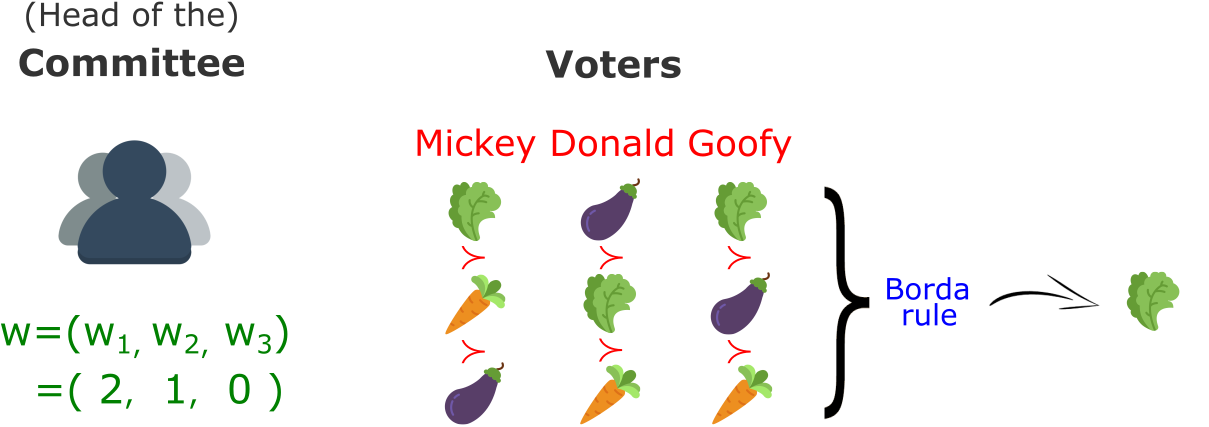
\includegraphics[scale=0.35]{classset.png}
%		%		\caption{.}
%		%		\label{fig:b1}
%	\end{figure}
%	\onslide<2-> \textbf{Goal}: Find a consensus choice 
%\end{frame}

\begin{frame}
\frametitle{Introducing the problem}
%\framesubtitle{Robust Winner Determination}
%	\textbf{Setting}: Two kind of players
\textbf{Setting}: Incompletely specified preferences and social choice rule \bigskip
\onslide<2-> \begin{figure}
	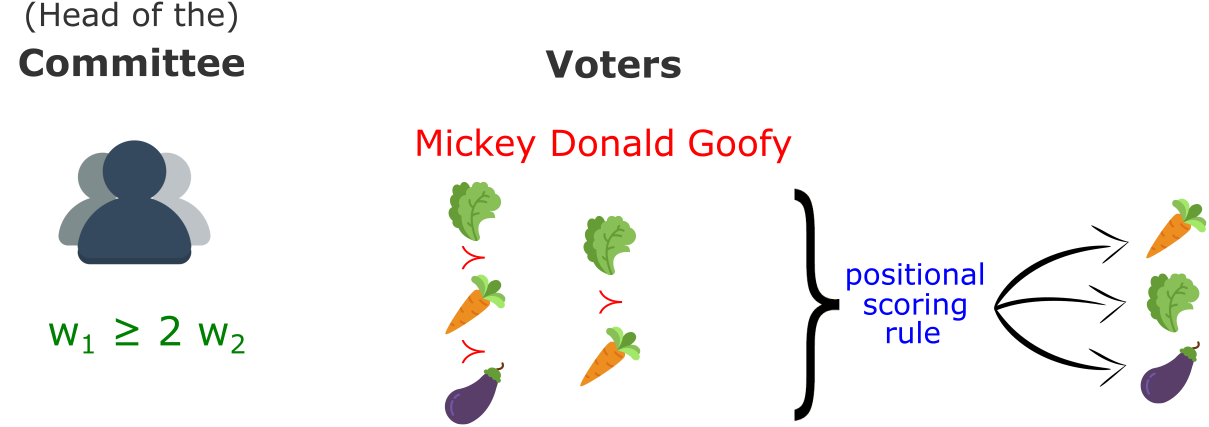
\includegraphics[scale=0.35]{ourset.png}
	%		\caption{.}
	%		\label{fig:b1}
\end{figure}
\onslide<3-> \textbf{Goal}: Develop an incremental elicitation strategy to quickly acquire the most relevant information 
\end{frame}
%\addtocounter{framenumber}{-1}
%\begin{frame}
%	\frametitle{Scenario}
%	\textbf{Setting}: Incompletely specified profile and positional scoring rule
%	\begin{figure}
%		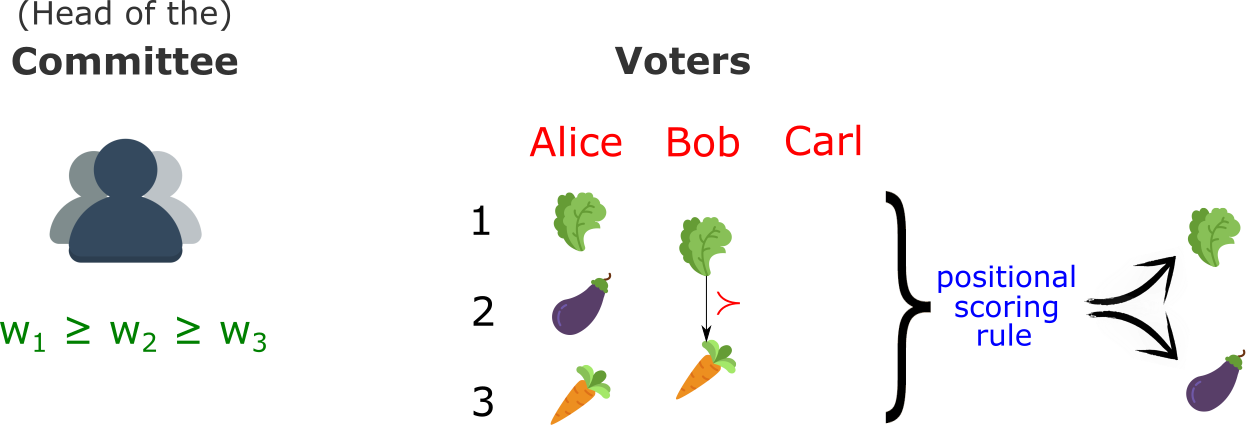
\includegraphics[scale=0.35]{set2.png}
%%		\caption{.}
%%		\label{fig:b1}
%	\end{figure}
%	\textbf{Goal}: Development of an incremental elicitation protocol based on minimax regret 
%\end{frame}

\begin{frame}
	\frametitle{Motivation and approach}
	\textbf{Who?}
	\begin{itemize}
		\item Imagine to be an \emph{external observer} helping with the voting procedure
	\end{itemize}
	\onslide<2-> \textbf{Why?}
	\begin{itemize}
		\item Voters: difficult or costly to order \emph{all} alternatives
		\item Committee: difficult to \emph{specify} a voting rule precisely
	\end{itemize}
	\onslide<3-> \textbf{What?}
	\begin{itemize}
		\item We want to reduce uncertainty, inferring (\textit{eliciting}) the true preferences of voters and committee, in order to quickly converge to an optimal
		or a near-optimal alternative
	\end{itemize}		
\end{frame}

\begin{frame}
	\frametitle{Motivation and approach}
	\onslide<1-> \textbf{Approach}
	\begin{itemize}
		\item Develop query strategies that interleave questions to the committee and questions to the voters
		\item Use \emph{Minimax regret} to measure the quality of those strategies
	\end{itemize}
	\onslide<2-> \textbf{Assumptions}
	\begin{itemize}
		\item We consider \textit{positional scoring rules}, which attach weights to positions according to a scoring vector $w$
		\item We assume $w$ to be \textit{convex}
		\[ w_r - w_{r+1} \geq w_{r+1}-w_{r+2} \qquad \forall r\]
		and that $w_1=1$ and $w_m=0$
	\end{itemize}	
\end{frame}

\subsection{Related Works}
\begin{frame}
	\frametitle{Related Works}
	\textbf{Incomplete profile}  
	\begin{itemize}
		\item and known weights: Minimax regret to produce a robust winner approximation (\textit{Lu and Boutilier 2011}, \cite{Lu2011}; \textit{Boutilier et al. 2006}, \cite{Boutilier2006})
	\end{itemize}~\\
	\textbf{Uncertain weights} 
	\begin{itemize}
		\item and complete profile: dominance relations derived to eliminate alternatives always less preferred than others (\textit{Stein et al. 1994}, \cite{Stein1994})
		\item in positional scoring rules (\textit{Viappiani 2018}, \cite{Viappiani2018})
	\end{itemize}
\end{frame}

\subsection{Notation}
\begin{frame}
	\frametitle{Notation}

		\begin{description}[$W=(\w_k,\ 1\leq k \leq m), \ W \in \mathcal{W}$]
			\item [$P \in \mathcal{P}$] complete preferences profile 
			\item [$W=(\w_r,\ 1\leq r \leq m), \ W \in \mathcal{W}$] (convex) scoring vector that the committee has in mind
		\end{description}
		\bigskip
		\onslide<2-> \begin{block}{}
			$W$ defines a Positional Scoring Rule $f_W(P)\subseteq \allalts$ using scores \color{blue}$s^{W,P}(a), \ \forall \ a \in \allalts$
		\end{block}
		\onslide<3-> \begin{block}{}
			$P$ and $W$ exist in the minds of voters and committee but unknown to us
		\end{block}
		
\end{frame}

\subsection{Questions}
\begin{frame}
	\frametitle{Questions}
	Two types of questions:\\
	\vspace{0.5cm}
	\onslide<2-> \textbf{Questions to the voters}
	\begin{itemize}
		\item[] Comparison queries that ask a particular voter to compare two alternatives $a, b \in \allalts$
		\color{blue}\[a \pref_j b \quad ?\]
	\end{itemize}
	\onslide<3->  \textbf{Questions to the committee}
	\begin{itemize}
		\item[] Queries relating the difference between the importance of consecutive ranks from $r$ to $r+2$
		\color{blue} \[ w_{r} - w_{r+1} \geq \lambda (w_{r+1} - w_{r+2}) \quad ? \] 
	\end{itemize}
\end{frame}

\subsection{Current Knowledge}
\begin{frame}
	\frametitle{Current Knowledge}
	The answers to these questions define $C_P$ and $C_W$ that is our knowledge about P and W 
	\medskip
	\begin{itemize}
		\onslide<2-> \item $C_P \subseteq \mathcal{P}$ constraints on the profile given by the voters
		\onslide<3-> \item $C_W \subseteq \mathcal{W}$ constraints on the voting rule given by the committee
	\end{itemize}

	\def\Pcircle{(0,0) circle (0.6cm)}
	\def\CPcircle{(0,0) circle (0.2cm)}
	\def\Wcircle{(0,-1.6) circle (0.6cm)}
	\def\CWcircle{(0,-1.6) circle (0.2cm)}
	\def\Allcircle{(3,-0.8) circle (0.6cm)}
	\def\Currcircle{(3,-0.8) circle (0.2cm)}
	\def\wcircle{(3,-0.8) circle (0.05cm)}
	\begin{center}
		\begin{tikzpicture}
			\onslide<2->\draw \Pcircle node[left] at (0,0.7) {\footnotesize$\mathcal{P}$};
			\onslide<2->\filldraw[fill=gray, draw=black] \CPcircle node[above]  at (0,0.07) {\footnotesize$C_P$};
			\onslide<3->\draw \Wcircle node[left] at (0,-0.9) {\footnotesize$\mathcal{W}$};
			\onslide<3->\filldraw[fill=gray, draw=black] \CWcircle node[above]  at (0,-1.5) {\footnotesize$C_W$};
			\onslide<4->\draw [decorate, decoration = {brace, raise=40pt, amplitude=5pt}] (0,0.7) --  (0,-2.3);
			\onslide<5->\draw \Allcircle node[above] at (3,-0.2) {\footnotesize$\powersetz{\allalts}$};
			\onslide<5->\filldraw[fill=gray, draw=black] \Currcircle node[above]  at (3,-0.7){\footnotesize$C_{\mathscr{P}}$};
			\onslide<6->\filldraw[fill=black, draw=black] \wcircle;
		\end{tikzpicture}
	\end{center}
\end{frame}

\subsection{Minimax Regret}
\begin{frame}
	\frametitle{Minimax Regret}
	Given $C_P \subseteq \mathcal{P}$ and $C_W \subseteq \mathcal{W}$:
	
	\begin{block}{}
		\[\color{red}{\PMR^{C_P,C_W}(a,b)}= \max_{P\in C_P, W \in C_W} s^{P,W}(b)-s^{P,W}(a) \]
		is the maximum difference of score between $a$ and $b$ under all possible realizations of the full profile {\em and} weights
	\end{block}
	
	\onslide<2->  We care about the worst case loss: \emph{maximal regret} between a chosen alternative $a$ and best real alternative $b$
	\[\MR^{C_P,C_W}(a)= \max_{b\in \allalts} \PMR^{C_P,C_W}(a,b) \]
	 	
	\onslide<3-> \centerline{\textbf{We select the alternative which \emph{minimizes} the maximal regret}}
	\[\MMR^{C_P,C_W}= \min_{a\in \allalts} \MR^{C_P,C_W}(a)\]
\end{frame}

\subsection{Pairwise Max Regret Computation}
\begin{frame}
	\frametitle{Pairwise Max Regret Computation}
	The computation of $\PMR^{C_P,C_W}( \icimg{salad.png},\icimg{aubergine.png})$ can be seen as a game in which an adversary both:
	\begin{itemize}
		\onslide<2-> \item \textbf{chooses a complete profile $\mathbf{P \in \mathcal{P}}$}\\
		\medskip
		\begin{center}
			
\includegraphics[scale=0.35]{completion4.png}
		\end{center}
		
		\onslide<3-> \item \textbf{chooses a feasible weight vector $\mathbf{W \in \mathcal{W}}$}\\
		\medskip
		\centerline{\color{red}$\mathbf{(1,?,0)}$ \icarr{arrow.png} \color{red}$\mathbf{(1,0,0)}$}
	\end{itemize}
	\medskip
	in order to maximize the difference of scores
\end{frame}

%\subsection{Computing Minimax Regret}
%\begin{frame}[t]
%	\frametitle{Computing Minimax Regret: Example}
%	\textbf{Profile completion}\\
%	Consider the following partial profile
%	\begin{center}
%		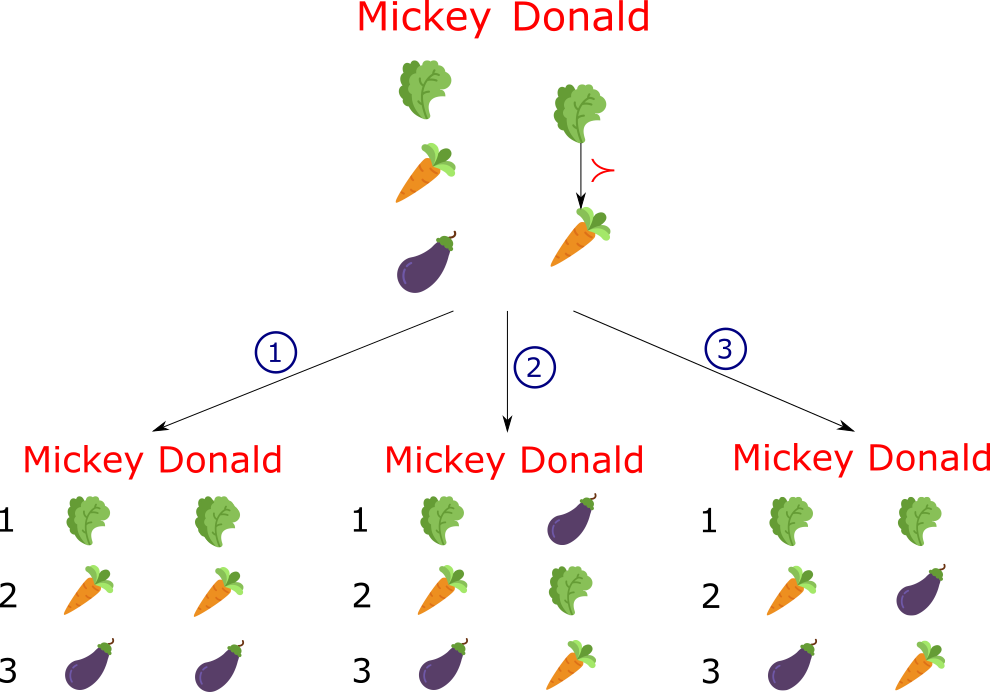
\includegraphics[scale=0.33]{compl.png}
%	\end{center}
%\end{frame}
%\begin{frame}[t]
%	\frametitle{Computing Minimax Regret: Example}
%	\textbf{Weight selection} \\ \bigskip
%	Consider the following constraint on the scoring vector given by the committee
%	\[w_1 \geq 2 \cdot w_2\]
%	and the convex assumption
%	\[w_1 - w_2 \geq w_2 - w_3 \]
%
%\end{frame}
%\begin{frame}[t]
%	\frametitle{Computing Minimax Regret: Example}
%	\textbf{Minimax computing}\\
%	\begin{center}
%		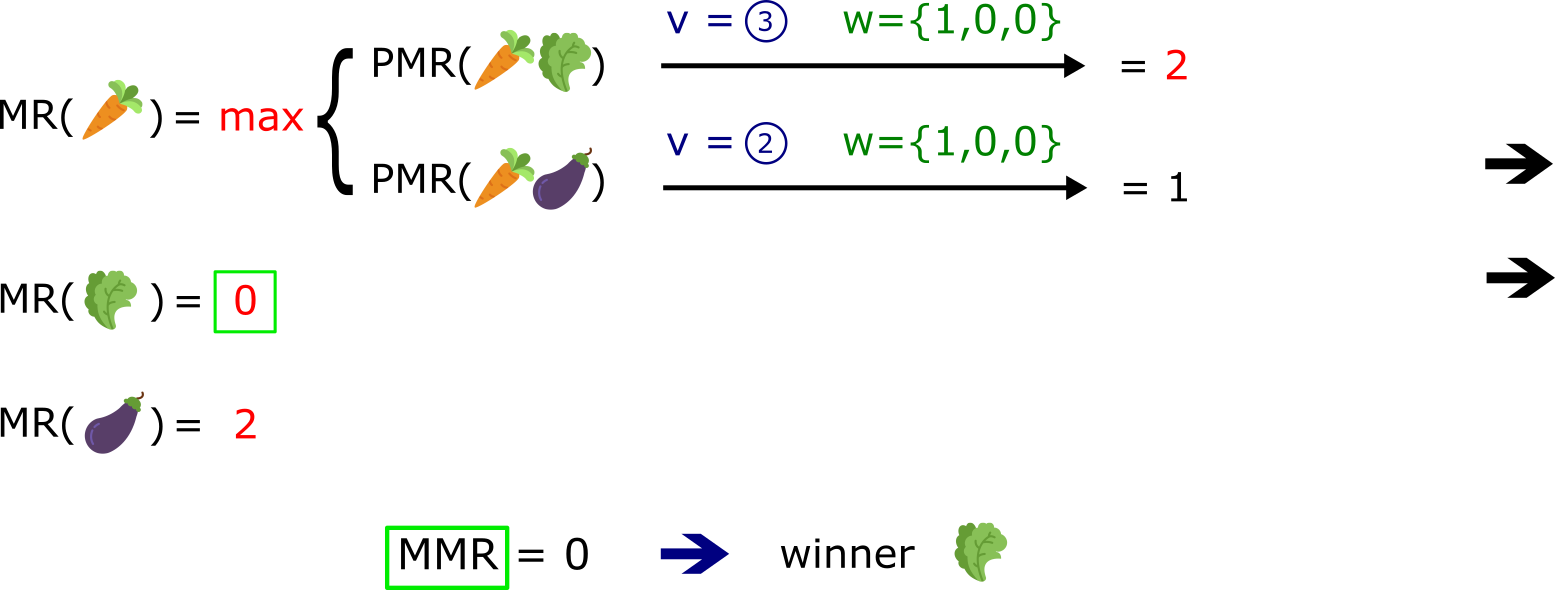
\includegraphics[scale=0.35]{minmax.png}
%	\end{center}
%\end{frame}

	
	\subsection{Elicitation strategies}
	\begin{frame}
		\frametitle{Elicitation strategies}
		At each step, the strategy selects a question to ask either to one of the voters about her preferences or to the committee about the voting rule \\ \bigskip
		\onslide<2-> The termination condition could be:
		\begin{itemize}
			\item <3-> when the minimax regret is lower than a threshold
			\item <4-> when the minimax regret is zero
		\end{itemize}
		\bigskip
	\end{frame}
	
	\begin{frame}[t]
		\frametitle{Elicitation strategies}
		\framesubtitle{Pessimistic Strategy}
		\onslide<1-> Assume that a question leads to the possible new knowledge states $(C_P^1, C_W^1)$ and $(C_P^2, C_W^2)$ depending on the answer, then the badness of the question in the worst case is:
		\[\max_{i=1,2} \MMR(C_P^i, C_W^i) \]
		\onslide<2-> The pessimistic strategy selects the question that leads to minimal regret in the worst case from a set of $n+1$ candidate questions \\
		\bigskip
		{\small \onslide<3-> \begin{block}{Note:}
			if the maximal MMR of two questions are equal, then prefers the one with the lowest MMR values associated to the opposite answer
		\end{block}}
	\end{frame}
	
	\begin{frame}
	\frametitle{Elicitation strategies}
	\framesubtitle{Pessimistic Strategy: Candidate questions}
	Let $(a^{*}, \bar{b}, \bar{P}, \bar{W})$ be the current solution of the minimax regret \\ \vspace{0.5em}
	We select $n + 1$	candidate questions:
	\begin{itemize}
		\item \textbf{One question per voter:} For each voter $i$, either:  
			\begin{itemize}
				\item $a^* \pref^{\bar{P}}_j \bar{b}$ : we ask about an incomparable alternative that can be placed above $a^*$ by the adversary to increase PMR($a^*$,$\bar{b}$)
				\item $\bar{b} \pref^{\bar{P}}_j a^*$: we ask about an incomparable alternative that can be placed between $a^*$ and $\bar{b}$ by the adversary to increase PMR($a^*$,$\bar{b}$) 
				\item $a^*$ and $\bar{b}$ are incomparable: we ask to compare them
		\end{itemize}
		\item \textbf{One question to the committee:} Consider $W_\tau$ the weight vector that minimize the PMR in the worst case. \\ We ask about the position
		$r = \argmax\limits_{i= [\![1, m-1]\!] } |\bar{W}(i)-W_\tau(i)|$
		
	\end{itemize}
	\end{frame}
	
	\subsection{Empirical Evaluation}
	\begin{frame}
		\frametitle{Empirical Evaluation}
		\framesubtitle{Pessimistic for different datasets}
		\begin{figure}
			\centering
			\caption{Average MMR (normalized by $n$) after $k$ questions with Pessimistic strategy for different datasets.}
			\label{fig:linearity}
			\begin{tikzpicture}
				\pgfplotsset{
					every axis legend/.append style={
						at={(0.5,1.1)},
						anchor=south
					},
				}
				\begin{axis}[
					y=80,
					legend columns=3,
					xlabel=Number of Questions,
					ylabel=MMR/n,
					ytick={0,0.5,1},
					xtick distance=100,
					xtick pos=left,
					ymajorgrids=true,
					enlarge x limits=-1, %hack to plot on the full x-axis scale
					width=10cm, %set bigger width
					ytick style={draw=none},
					ymin=0,
					ymax=1,
					xmin=0,
					xmax=1000,
					yticklabels={0,0.5,1},
					legend style={font=\footnotesize}]
					
					\addlegendimage{mark=halfsquare right*,brown,mark size=2}
					\addlegendimage{mark=diamond*,red,mark size=2}
					\addlegendimage{mark=pentagon*,cyan,mark size=2}
					\addlegendimage{mark=halfcircle*,violet,mark size=2}
					\addlegendimage{mark=*,pink,mark size=2}
					\addlegendimage{mark=triangle*,green,mark size=2}
					\addlegendimage{mark=halfsquare left*,blue,mark size=2}
					\addlegendimage{mark=square*,teal,mark size=2}
					\addlegendimage{mark=halfsquare*,magenta,mark size=2}
					
					
					\addplot[thick, mark=halfsquare right*, mark size = {2}, mark indices = {120}, brown] table [x=k, y=5.20]{data/linearity.dat};
					\addlegendentry{m=5, n=20}
					\addplot[thick, mark=diamond*, mark size = {2}, mark indices = {150}, red] table [x=k, y=10.20]{data/linearity.dat};
					\addlegendentry{m=10, n=20}
					\addplot[thick, mark=pentagon*, mark size = {2}, mark indices = {240}, cyan] table [x=k, y=11.30]{data/linearity.dat};
					\addlegendentry{m=11, n=30}
					\addplot[thick, mark=halfcircle*, mark size = {2}, mark indices = {400}, violet] table [x=k, y=tshirts]{data/linearity.dat};
					\addlegendentry{tshirts m11n30}
					\addplot[thick, mark=*, mark size = {2}, mark indices = {400}, pink] table [x=k, y=courses]{data/linearity.dat};
					\addlegendentry{courses m9n146}
					\addplot[thick, mark=triangle*, mark size = {2}, mark indices = {400}, green] table [x=k, y=9.146]{data/linearity.dat};
					\addlegendentry{m=9, n=146}
					\addplot[thick, mark=halfsquare left*, mark size = {2}, mark indices = {200}, blue] table [x=k, y=14.9]{data/linearity.dat};
					\addlegendentry{m=14, n=9}
					\addplot[thick, mark=square*, mark size = {2}, mark indices = {60}, teal] table [x=k, y=skate]{data/linearity.dat};
					\addlegendentry{skate m14n9}
					\addplot[thick, mark=halfsquare*, mark size = {2}, mark indices = {400}, magenta] table [x=k, y=15.30]{data/linearity.dat};
					\addlegendentry{m=15, n=30}
				\end{axis}
			\end{tikzpicture}
		\end{figure}
	\end{frame}
	
	\begin{frame}
		\frametitle{Empirical Evaluation}
		\framesubtitle{Pessimistic reaching "low enough" regret}
		\sisetup{table-number-alignment = center, table-figures-integer=2, table-figures-decimal=1, table-auto-round}
		\begin{minipage}{\textwidth}
			\captionof{table}{Questions asked by Pessimistic strategy on several datasets to reach $\frac{n}{10}$ regret, columns 4 and 5, and zero regret, last two columns.}
			\label{tab:questions}
			\scalebox{0.8}{
			\begin{tabular}{cccS[table-number-alignment = center, table-figures-integer=2] S[table-figures-integer=3, table-figures-decimal=1]@{ | }S[table-figures-integer=2, table-figures-decimal=1]@{ | }S[table-figures-integer=2, table-figures-decimal=1]@{ ]} S[table-number-alignment = center, table-figures-integer=2]S[table-figures-integer=3, table-figures-decimal=1]@{ | }S[table-figures-integer=2, table-figures-decimal=1]@{ | }S[table-figures-integer=2, table-figures-decimal=1]@{ ]}}
				\toprule
				{dataset} & m & n &{$q_{c}^{\scriptscriptstyle{MMR} \leq n/10}$} & \multicolumn{3}{c}{$q_{a}^{\scriptscriptstyle{MMR} \leq n/10}$} & {$q_{c}^{ \scriptscriptstyle{MMR} = 0}$} & \multicolumn{3}{c}{$q_{a}^{ \scriptscriptstyle{MMR} = 0}$} \\
				\midrule
				m5n20 & 5&20&0.0&[4.3 &4.95 & 5.84 &5.25&[ \ 5.36 & 6.15 & 7.21\\
				m10n20&10&20&0.0&[13.85 & 16.1& 18.41&31.95&[19.66 & 21.78 & 24.7\\
				m11n30&11&30&0.0&[16.55&19.0&22.26&45.15&[23.07&25.7&28.89\\
				tshirts&11&30&0.0&[13.08&16.6&19.58& 43.15 &[28.22&31.98 &35.62\\
				courses&9&146&0.0&[6.03 &7.0 &7.0&0.0&[6.81 & 7.0 &7.0\\
				%m9n146&9&146&0&0&[1.94 &8 &9.25&999.3&0.47&0&0&[1.94&8&9.25&999.3&0.47\\
				m14n9&14&9&5.4&[30.3&33.45&36.65&64.05&[37.55&40.5&44.3\\
				skate&14&9&0.0&[11.35&11.6&12.3&0.0&[11.5&11.8&12.75 \\
				m15n30&15&30&0.0&[24.95&29.5&33.68 \\
				\bottomrule
			\end{tabular}}
		\end{minipage}
	\end{frame}


\begin{frame}
	\frametitle{Empirical Evaluation}
	\framesubtitle{Pessimistic committee first and then voters (and vice-versa)}
	\sisetup{table-number-alignment = center, table-figures-integer=2, table-figures-decimal=1, table-auto-round}
	\begin{minipage}{\textwidth}
		\centering
		\captionof{table}{Average MMR in problems of size $(10, 20)$ after $500$ questions, among which $q_c$ to the chair.}
		\label{tab:twoP500}
		\scalebox{0.85}{
			\begin{tabular}{S[table-figures-integer=3, table-figures-decimal=0]S[table-number-alignment = right]@{ ± }S[table-number-alignment = left, table-figures-integer=1]S[table-number-alignment = right]@{ ± }S[table-number-alignment = left, table-figures-integer=1]}
				\toprule
				{$q_c$} & {2 ph.\ ca} & {sd} & {2 ph.\ ac} & {sd} \\
				\midrule		
				
				0	&	0.62	&	0.52	&	0.62	&	0.52	\\
				15	&	0.515	&	0.48	&	0.54	&	0.46	\\
				30	&	0.345	&	0.47	&	0.325	&	0.425	\\
				50	&	0.045	&	0.09	&	0.03	&	0.065	\\
				100	&	0.14	&	0.23	&	0.075	&	0.135	\\
				200	&	2.305	&	1.36	&	2.145	&	1.845	\\
				300	&	5.15	&	2.38	&	6.83	&	0.625	\\
				400	&	10.905	&	0.89	&	12.245	&	0.99	\\
				500	&	20.0	&	0.0	&	20.0	&	0.0	\\
				
				\bottomrule
			\end{tabular}
		}
	\end{minipage}
\end{frame}


\section{Preference Elicitation under Majority Judgment}
\subsection{Context}
\begin{frame}
	\frametitle{Context}
	\framesubtitle{Introducing the problem}
	\textbf{Setting}: Voters judges a random subset of alternatives and the preferences are aggregated with the Majority Judgment rule \vspace{6mm}
	
	\onslide<2->{\textbf{Goal}: Analyse the impact of the randomness in the result and find a more efficient elicitation procedure}
\end{frame}

\begin{frame}
	\frametitle{Context}
	\framesubtitle{Majority Judgment}
		Voters judges candidates assigning grades from an ordinal scale. The winner is the candidate with the highest median of the grades received. \vspace{1cm} \\
	
\includegraphics[width=\textwidth]{vector}
\end{frame}

\begin{frame}
	\frametitle{\textbf{Current Work:} Preference Elicitation under Majority Judgment}
	\framesubtitle{Introducing the problem}
	\onslide<1-> In the last few years MJ has being adopted by a progressively larger number of french political parties including: Le Parti Pirate, Génération(s), LaPrimaire.org, France Insoumise and La République en Marche. \vspace{1cm}
	
	\onslide<2-> LaPrimaire.org is a french political initiative whose goal is to select an independent candidate for the french presidential election using MJ as voting rule.
\end{frame}

\begin{frame}
	\frametitle{\textbf{Current Work:} Preference Elicitation under Majority Judgment}
	\framesubtitle{LaPrimaire.org}
	The procedure consists of two rounds:
	\begin{itemize}
		\item[1:]<2-> each voter expresses her judgment on five random candidates. The five ones with the highest medians qualify for the second round. 
		\item[2:]<3-> each voter expresses her judgment on all the five finalists. The one with the best median is the winner.
	\end{itemize}
\end{frame}

\subsection{Research Questions}
\begin{frame}
	\frametitle{\textbf{Current Work:} Research Questions}
	\begin{itemize}
		\item<1-> Does expressing judgment on random candidates influence the result? 
		\item<2-> Does the number of questions influence the result? 
		\item<3-> What is the best trade-off between communication cost and optimal result?
		\item<4-> What is the voting rule applied on the resulting incomplete profile? What are its properties?
		\item<5-> The random selection of questions is fair in terms of probability of being asked about a certain candidate $i$, but is it fair in terms of $i$ being elected?
		\item<6-> Can we select the next question using a minimax regret notion instead of randomly selecting a candidate?
		\item<7-> Suppose that the fraction of candidates that each voter judges is variable, how this rule differ from the previous one? Can a voter manipulate the result by judging only certain candidates?
	\end{itemize}
\end{frame}


\addtocounter{framenumber}{-1}
\begin{frame}[plain]
	\centering \color{darkred}\LARGE Thank You!
\end{frame}

\begin{frame}
	\frametitle{Plan of the thesis and questions}
	\begin{itemize}
		\item Final dissertation by October 2021, defense by December 2021
		\item Status of the works:
		\begin{itemize}
			\item Compromise: Rejected from Social Choice and Welfare; under submission to Review of Economic Design;
			\item Elicitation PSR: Rejected from IJCAI20, AAMAS21 and IJCAI21; under revision at ADT21;
			\item Elicitation MJ: ongoing work, plan to have a final draft before the defense.
		\end{itemize}
		\item Given the current status of my works, is the plan feasible?
		\item Any suggestions on the dissertation structure ?
	\end{itemize}
\end{frame}


\bibliographystyle{plain}
\bibliography{biblio} 
%given a combination of axioms we want to find an outcome that doesn't satisfy them, and we would do that for several reasons:
%-querying the user, depending of her answer we might infer her preferences over the set of axioms;
%-proving that a set of axioms is not valid giving a counter-example;


%A method for automatically proving impossibility theorems in the area of ranking sets of objects has already been implemented (Geist \& Endriss, 2011). It:



\end{document}